\documentclass[a4paper]{article}
\usepackage[english]{babel}
\usepackage[utf8x]{inputenc}
\usepackage{amsmath}
\usepackage{graphicx}
\usepackage[colorinlistoftodos]{todonotes}

\title{Assignment 1: Search Algorithms Report}
\author{Stephen Weinpahl (sjw170) and Michael Trinh (mht46)}
\date{}

\begin{document}
\maketitle
\section*{{Preface}}

\textit
{The searching python file contains five complete searching algorithms to find a path from the start point to the end point in the maze. An initial problem file provides the maze number which relates to a file that describes the maze’s structure, the start and end points and the algorithm which is used to solve the maze. The included python file needs all related maze files to be included in the same directory that the python file is in. The files methods as well as their purpose are described in the readme. Several libraries were used to assist in the implementation of the algorithms and visualization, including the deque library from collections which implements a queue, the heapq library which implements a min heap and the matplotlib and numpy libraries which implement the maze and data visualization. This report will focus on comparing several well known algorithms performance on solving the maze and will look to explain their behavior. }
\newline
\newline
\section*{{Problem Description}}
\begin{itemize}
    \item States: Location of the agent on a grid.
    \item Initial State: The initial state is a point on the grid that the agent starts at.
    \item Goal State: Reaching a specific cell in the grid without colliding with any blocked cells.
    \item Actions: The agent can move left, right, up, or down, but cannot move diagonally.
    \item Transition Model: The result of moving to a cell.
    \item Action Cost: Moving left/right has an action cost of 1, and moving up/down has an action cost of 2.
    \item Observability: Full observability of the maze as all the cell values are known
    \item The model is deterministic as the outcome can be determined based on a specific state (assuming a non stochastic heuristic is applied)
    \item The problem is discrete, complete and sequential
\end{itemize}

\begin{figure}
    \section*{{Setup}}
    \centering
    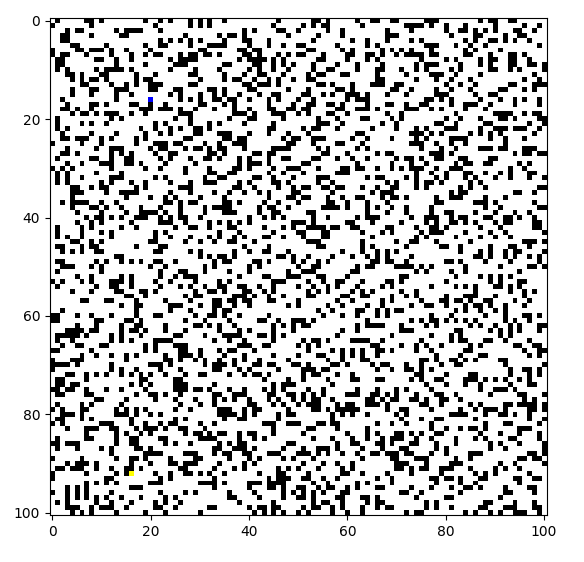
\includegraphics[width=0.75\textwidth]{fig1.png}
    \caption{Maze000 Initial Conditions}
    \label{fig:Maze000}
\end{figure}

Our solution contains a method called showInitialMaze which takes in a file of the format of problem.txt and builds a maze object and visualizes the maze with the start and end points and black boxes as the barriers. An example of maze000.txt with a start point of (16, 20) and a goal of (92, 16) is shown below where blue is the start point and yellow is the goal point. 
\newpage

\section*{{Analysis}}
\textit{1. Algorithm 0: Uniform Cost Search}
\begin{itemize}
    \item Completeness: UCS is considered complete, as it will consider all paths systematically, in order of increasing cost, never getting caught going down a single infinite path.
    \item Optimal: UCS is optimal as the first solution it finds will have a cost at least as low as the cost of any other node in the frontier.
    \item Comparison to Breadth-First Search: Similar to UCS, BFS is considered complete as it will generate all possible paths, thus if one of these paths are a solution, it will be found. However, it is only cost optimal when every action costs the same. Thus, BFS will not be optimal for our problem.
\end{itemize}
Running the UCS algorithm on the initial problem described in the setup above, the following path is found. It has a cost of 176 and took .0217 seconds to compute. The red cells are all the visited cells and the green shows the path from start state to the goal state.
\begin{figure}[ht]
    \centering
    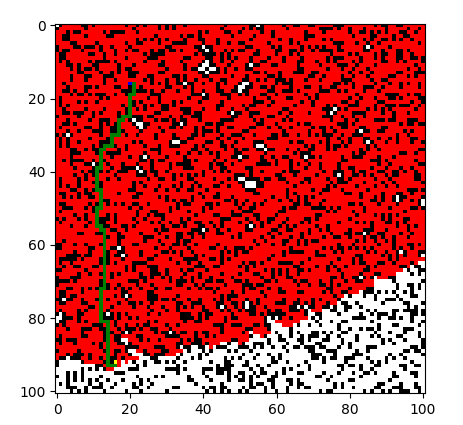
\includegraphics[width=0.75\textwidth]{fig2.png}
    \caption{Uniform Cost Search on Initial Problem}
    \label{fig:UCS}
\end{figure}
\newline
Looking at the area the algorithm searches, it actually covers a relatively large amount of the maze before finding the optimal path. This is due to the min heap that is used to sort by cost, meaning that nodes that are far away from the goal will still be considered if their cost is low enough. Compared to some algorithms that consider heuristics such as A*, this could become inefficient as the size of the maze and the distance between the start and goal stats becomes very large.

\newpage

\textit{2. Algorithm 1: Iterative Deepening Depth-First Search}
\begin{itemize}
    \item Completeness: IDDFS is considered complete since our problem is a finite space and returns a solution if one exists.
    \item Optimal: IDDFS is not optimal for this problem since the cost of some actions are different.
\end{itemize}
Running the IDDFS algorithm on the initial problem described in the setup above, the following path is found. It has a cost of 784 and took 2.577 seconds to compute. The red cells are all the visited cells and the green shows the path from start state to the goal state.

\begin{figure}[ht]
    \centering
    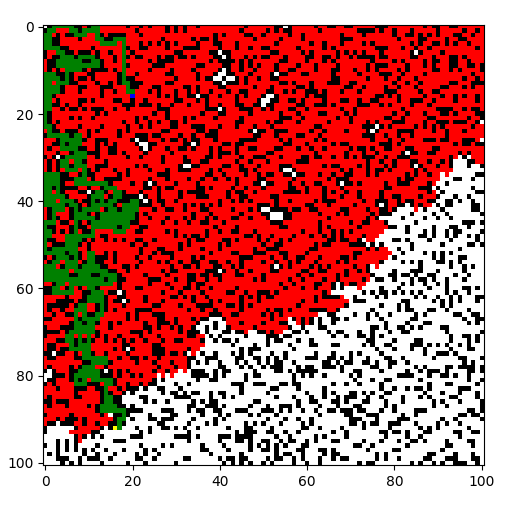
\includegraphics[width=0.75\textwidth]{fig3.png}
    \caption{Iterative Deepening Depth-First Search on Initial Problem}
    \label{fig:IDDFS}
\end{figure}

Comparing the searched area from IDDFS to UCS, it appears that IDDFS searches less of the maze despite taking far more time than UCS. This is because it iterates through the Depth Limited Search algorithm, incrementing the max depth by 1 each time the search fails untils it hits a maximum allowable depth. Because of this it is actually running the Depth Limited Search for many iterations before finding a solution. Another issue is that the DLS algorithm does not find an optimal solution as the path is randomly determined by the specific order in which DLS searches its neighbors. Thus, the path is often much more complicated than it should be, however the path does not form cycles or overlap itself. The cost found for this algorithm is extremely high at 784, showing that this algorithm is probably not the best one to choose. Perhaps it could be useful if the max travelable distance was known before solving the problem, thus the algorithm would terminate after it could not find a solution that satisfies the cost constraint while other algorithms would continue searching.

\newpage

\textit{3. Algorithm 2: A* with Manhattan distance $(h_1)$}
\begin{itemize}
    \item Consistent: For our problem, A* Using Manhattan distance is considered consistent, as the first time we reach a new state, we are guaranteed to be on an optimal path. Thus, the function h(n) never becomes greater than the cost of the action from n to n’ plus the heuristic estimate.
    \item Admissible: Since the heuristic takes into account each individual cell when calculating costs, it will never make an overestimation.
\end{itemize}
Running the A* algorithm with manhattan distance as the heuristic on the initial problem described in the setup above, the following path is found. It has a cost of 176 and took .0154 seconds to compute. The red cells are all the visited cells and the green shows the path from start state to the goal state.

\begin{figure}[ht]
    \centering
    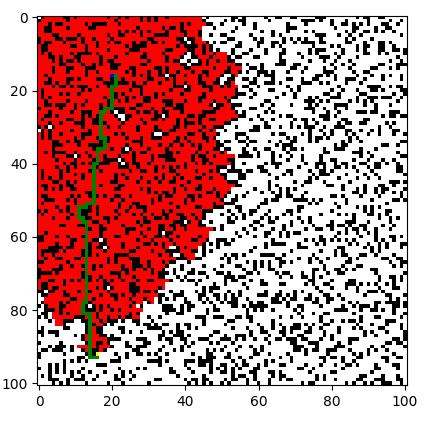
\includegraphics[width=0.75\textwidth]{fig4.png}
    \caption{A* using Manhattan Distance on Initial Problem}
    \label{fig:h1}
\end{figure}

\newpage

\textit{4. Algorithm 3: A* with Manhattan distance $(h_3)$}
\begin{itemize}
    \item Consistent: This algorithm uses either the euclidean distance or Manhattan distance to a goal state, whichever one is smaller. We have already shown that Manhattan distance is consistent. Euclidean distance is also consistent for a reason similar to Manhattan.
    \item Admissible: The Manhattan distance heuristic has already been shown to be admissible. Euclidean distance heuristic is also known to be admissible as it calculates a direct path to the goal, ignoring any barricades or even invalid paths and actions. As such, the cost to the path will never be overestimated.
\end{itemize}
Running the A* algorithm with the minimum of the Manhattan and euclidean distance as the heuristic on the initial problem described in the setup above, the following path is found. It has a cost of 176 and took .0218 seconds to compute. The red cells are all the visited cells and the green shows the path from start state to the goal state.

\begin{figure}[ht]
    \centering
    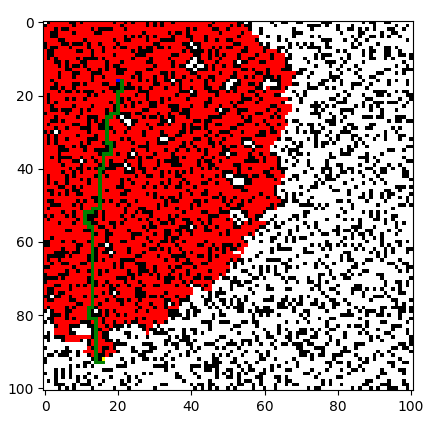
\includegraphics[width=0.75\textwidth]{fig5.png}
    \caption{A* using Minimum of Euclidean and Manhattan Distance on Initial Problem}
    \label{fig:h3}
\end{figure}

\textit{5. Algorithm 4: A* with custom heuristic}
\begin{itemize}
    \item Consistent: 
    \item Admissible: The heuristic takes the minimum of a randomly (between 0.0 and 1.0) scaled Manhattan and Euclidean distance heuristic. As such, the heuristic is only ever as big as either its Manhattan or Euclidean counterpart. With this being the case, the estimated costs will always be smaller than the actual costs. Thus, the custom heuristic is admissible.
    \item Explanation:
    \item Better than others?: As shown in the results, this heuristic actually performs about the same as other implemented heuristics. It neither performs worse or better than any of the others.
\end{itemize}
Running the A* algorithm with the custom heuristic on the initial problem described in the setup above, the following path is found. It has a cost of 176 and took .0335 seconds to compute. The red cells are all the visited cells and the green shows the path from start state to the goal state.


\begin{figure}[ht]
    \centering
    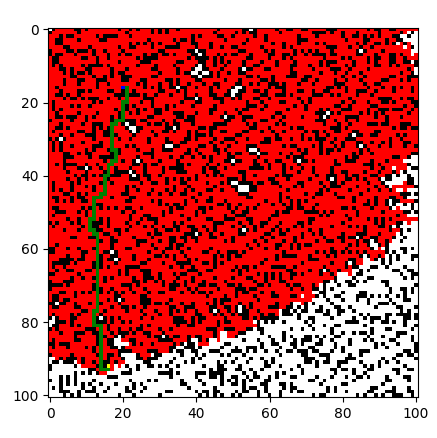
\includegraphics[width=0.75\textwidth]{fig6.png}
    \caption{A* using Custom Heuristic on Initial Problem}
    \label{fig:custom}
\end{figure}

\newpage

\section*{{Results}}
\begin{figure}[ht]
    \centering
    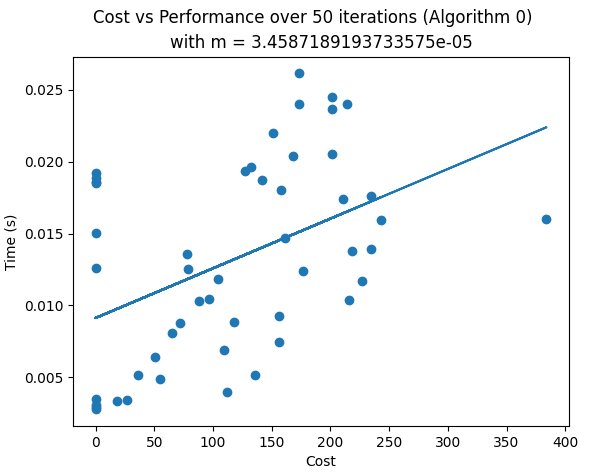
\includegraphics[width=\textwidth]{CVPALG0.png}
    \caption{Cost vs Performance over 50 iterations using Uniform Cost Search}
    \label{fig:CostVsPerformanceAlg0}
\end{figure}
\newpage
\begin{figure}[ht]
    \centering
    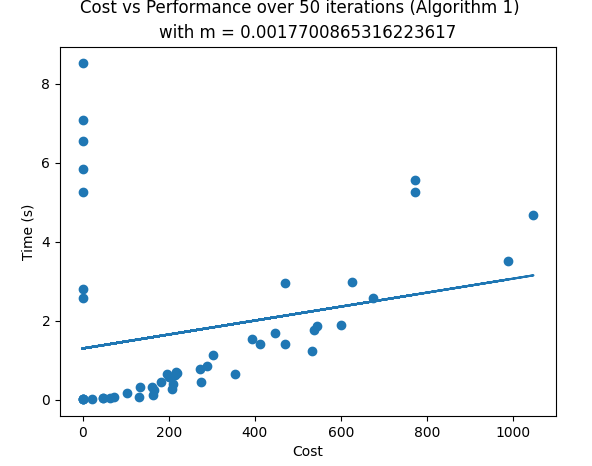
\includegraphics[width=\textwidth]{CVPALG1.png}
    \caption{Cost vs Performance using Iterative Deepening Depth First Search}
    \label{fig:CostVsPerformanceAlg1}
\end{figure}
\newpage
\begin{figure}[ht]
    \centering
    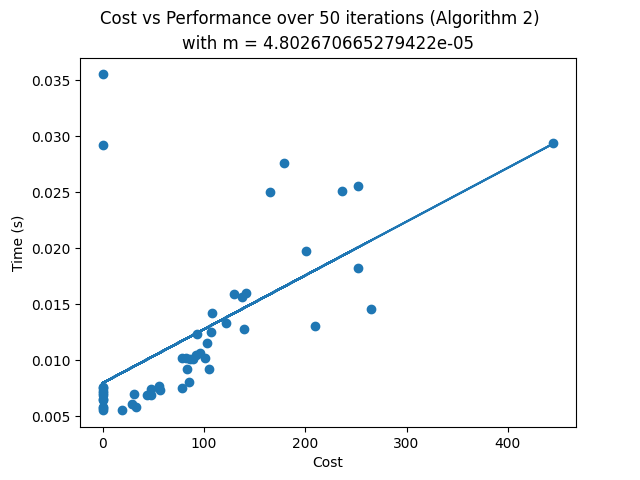
\includegraphics[width=\textwidth]{CVPALG2.png}
    \caption{ Cost vs Performance over 50 iterations using A* with Manhattan Distance}
    \label{fig:CostVsPerformanceAlg2}
\end{figure}
\newpage
\begin{figure}[ht]
    \centering
    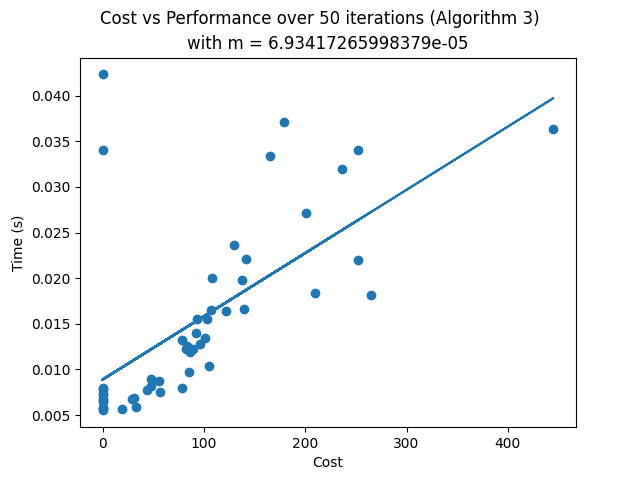
\includegraphics[width=\textwidth]{CVPALG3.png}
    \caption{Cost vs Performance using A* with min(Manhattan,Euclidean)}
    \label{fig:CostVsPerformanceAlg3}
\end{figure}
\newpage
\begin{figure}[ht]
    \centering
    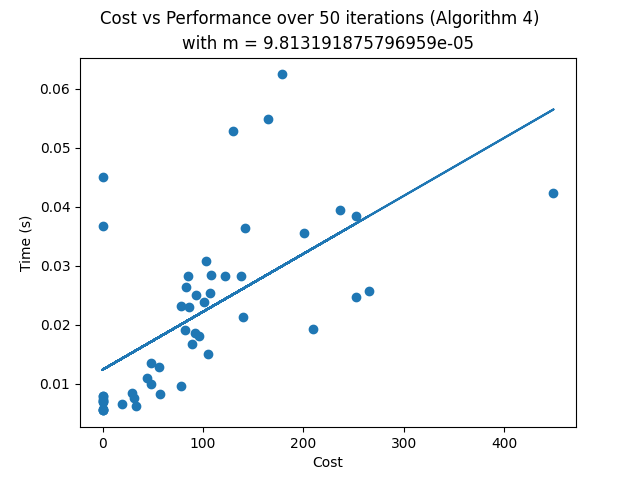
\includegraphics[width=\textwidth]{CVPALG4.png}
    \caption{Cost vs Performance using A* with custom heuristic}
    \label{fig:CostVsPerformanceAlg4}
\end{figure}
\newpage
\begin{figure}[ht]
    \centering
    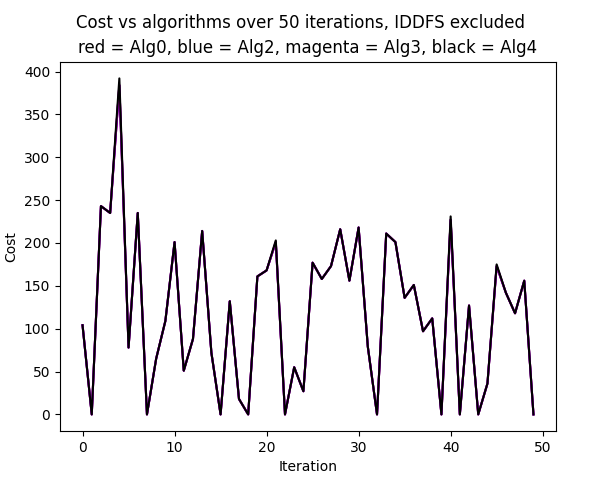
\includegraphics[width=\textwidth]{CVA50N.png}
    \caption{Cost vs Algorithm, Iterative Deepening Depth First Search excluded}
    \label{fig:CostVsAlgs}
\end{figure}
For this graph, we intentionally excluded IDDFS. The reason for this is due to how much of an outlier data from IDDFS produces. In any case, from this graph, we see that despite using different heuristics, all of the A* search algorithms performed with the same cost. Additionally, using Uniform Cost Search, an uninformed search algorithm, also shared the same cost as A*. From this, we gather not only that UCS is as cost optimal compared to an informed search algorithm, but that it is also as consistent as well.
\newpage
\begin{figure}[ht]
    \centering
    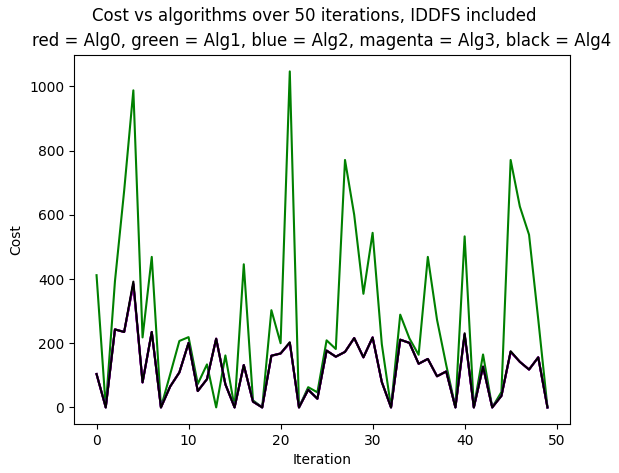
\includegraphics[width=\textwidth]{CVA50IDDFS.png}
    \caption{Cost vs Algorithms, including Iterative Deepening Depth First Search}
    \label{fig:CostVsAlgsIDDFS}
\end{figure}
For completeness, we have included IDDFS this time. As shown, IDDFS far exceeds the cost used compared to other algorithms implemented. Compared to other algorithms, IDDFS takes far longer, and costs much more despite searching less cells.

\end{document}